%% magick convert -density 1200 test.pdf test.png
\documentclass[preview, border={0.4pt 5pt 0.4pt 1pt}, varwidth=20cm]{standalone} % border options are {left bottom right top}

\usepackage[T1]{fontenc}
% \usepackage[sfdefault]{AlegreyaSans}
% \renewcommand*\oldstylenums[1]{{\AlegreyaSansOsF #1}}

\usepackage[sfdefault]{FiraSans} %% option 'sfdefault' activates Fira Sans as the default text font
\usepackage[T1]{fontenc}
\renewcommand*\oldstylenums[1]{{\firaoldstyle #1}}

% \usepackage[T1]{fontenc}
% \usepackage{Alegreya} %% Option 'black' gives heavier bold face 
% \renewcommand*\oldstylenums[1]{{\AlegreyaOsF #1}}


% \usepackage[default]{lato}
% \usepackage[T1]{fontenc}

% \usepackage[sfdefault]{cabin}
% \usepackage[T1]{fontenc}

% \usepackage[sfdefault]{roboto}  %% Option 'sfdefault' only if the base font of the document is to be sans serif
% \usepackage[T1]{fontenc}

% \usepackage[sfdefault]{noto}
% \usepackage[T1]{fontenc}

% \usepackage[T1]{fontenc}
% \usepackage[sfdefault]{josefin}

\usepackage{amsthm}
\usepackage{amssymb}
\usepackage{amsmath}
\usepackage{bm}
\usepackage{nicefrac}
\usepackage{graphicx}
\usepackage{tikz}
\usepackage{booktabs}
\usepackage{soul}

\usetikzlibrary{automata, positioning}

%% Colors
% grey
\definecolor{DarkCharcoal}{RGB}{30, 30, 30} % theorem
\definecolor{Davys}{RGB}{60, 60, 60} % proof
\definecolor{SonicSilver}{RGB}{90, 90, 90} % proposition
\definecolor{Gray}{RGB}{120, 120, 120} % lemma
\definecolor{Spanish}{RGB}{150, 150, 150} % corollary
\definecolor{Argent}{RGB}{180, 180, 180} % example

% blues
\definecolor{Azure}{RGB}{0, 128, 255}
\definecolor{Egyptian}{RGB}{16, 52, 166}
\definecolor{Navy}{RGB}{17, 30, 108}
\definecolor{CeruleanFrost}{RGB}{104, 145, 195}
\definecolor{LightSteelBlue}{RGB}{170, 197, 226}

% reds
\definecolor{Renate}{RGB}{227, 25, 113}
\definecolor{Burgundy}{RGB}{141, 2, 31}
\definecolor{Salmon}{RGB}{250, 128, 114}

% yellows
\definecolor{Honey}{RGB}{235, 150, 5}

% greens
\definecolor{PastelGreen}{HTML}{6ECB63}
\definecolor{FernGreen}{HTML}{116530}
\definecolor{CadmiumGreen}{HTML}{046C41}


%% Color Schemes
% Pastel Tones Color Scheme
\definecolor{Manatee}{RGB}{154, 145, 172} % darkest
\definecolor{Lilac}{RGB}{202, 167, 189}
\definecolor{CherryBlossomPink}{RGB}{255, 185, 196}
\definecolor{LightRed}{RGB}{255, 211, 212}

% Luxury Gradient Color Scheme
\definecolor{PhilippineBronze}{RGB}{112, 54, 14}
\definecolor{GoldenBrown}{RGB}{147, 93, 35}
\definecolor{UniversityOfCaliforniaGold}{RGB}{182, 131, 55}
\definecolor{Sunray}{RGB}{217, 170, 76}
\definecolor{OrangeYellowCrayola}{RGB}{252, 208, 96}

% Breaking Apart Color Scheme
\definecolor{DeepTuscanRed}{RGB}{103, 74, 82}
\definecolor{FuzzyWuzzy}{RGB}{199, 114, 113}
\definecolor{MiddleYellowRed}{RGB}{232, 187, 109}
\definecolor{Independence}{RGB}{83, 70, 103}
\definecolor{CeladonGreen}{RGB}{47, 129, 133}

% Lilac
\definecolor{Lilac1}{HTML}{97cded} % blue
\definecolor{Lilac2}{HTML}{02a0da}
\definecolor{Lilac3}{HTML}{b8afc9} % purple
\definecolor{Lilac4}{HTML}{eae1ef}
\definecolor{Lilac5}{HTML}{eadbd7} % light coffee

% Monochrome Coffee
\definecolor{MonoCoffee1}{HTML}{281E15} % dark
\definecolor{MonoCoffee2}{HTML}{47423E}
\definecolor{MonoCoffee3}{HTML}{928477}
\definecolor{MonoCoffee4}{HTML}{B7B2AC}
\definecolor{MonoCoffee5}{HTML}{A49FA3} % light

% Monochrome Amethyst
\definecolor{MonoAmethyst1}{HTML}{22222E} % dark
\definecolor{MonoAmethyst2}{HTML}{393A5A}
\definecolor{MonoAmethyst3}{HTML}{706F8E}
\definecolor{MonoAmethyst4}{HTML}{ADA9BA}
\definecolor{MonoAmethyst5}{HTML}{E9E9E9} % light

% Warm Brown
\definecolor{WarmBrown1}{HTML}{3C0906} % dark
\definecolor{WarmBrown2}{HTML}{84352D}
\definecolor{WarmBrown3}{HTML}{BC5F41}
\definecolor{WarmBrown4}{HTML}{E4E4E6}
\definecolor{WarmBrown5}{HTML}{E4C08A} % light

% FMAS course
\definecolor{GameTheory}{HTML}{AA2B1D}
\definecolor{Voting}{HTML}{FE9801}
\definecolor{Matching}{HTML}{F9B384}
\definecolor{Auctions}{HTML}{583D72}
\definecolor{ABMs}{HTML}{374045}
\definecolor{WisdomOfCrowds}{HTML}{7189BF}

% environments
\definecolor{colorTheorem}{HTML}{DA2D2D}
\definecolor{colorProposition}{HTML}{FF5733}
\definecolor{colorProof}{HTML}{621055}
\definecolor{colorDefinition}{HTML}{FF9F45}
\definecolor{colorAxiom}{HTML}{506D84}
\definecolor{colorProcedure}{HTML}{753422}
\definecolor{colorProblem}{HTML}{374045}
\definecolor{colorObservation}{HTML}{EA9ABB}
\definecolor{colorABM}{HTML}{89B5AF}
\definecolor{colorExample}{HTML}{97C4B8}
\definecolor{colorConjecture}{RGB}{217, 170, 76}


\newcommand{\EXP}{\mathbb{E}}
\newcommand{\maj}{{\textit{maj}}}
\renewcommand{\epsilon}{\varepsilon}


\tikzset{
  state/.style={
    circle,
    draw,
    minimum size=1cm,
    font=\small,
    align=center
  }
}

\begin{document}
    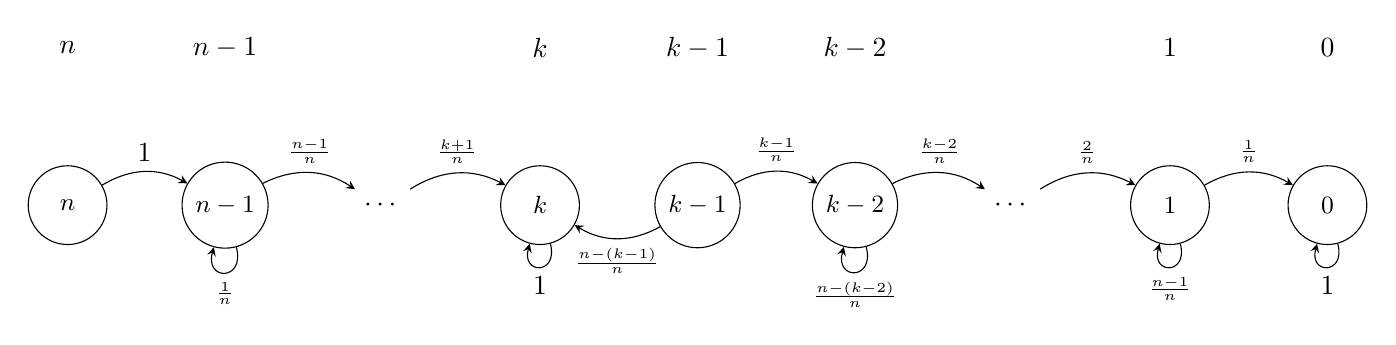
\begin{tikzpicture}[->, >=stealth, node distance=2cm, auto]
        % Define the nodes
        \node[state] (n)     {$n$};
        \node[state] (n1)    [right of=n] {$n-1$};
        \node        (dots)  [right of=n1] {$\cdots$};
        \node[state] (k)     [right of=dots] {$k$};
        \node[state] (k1)    [right of=k] {$k-1$};
        \node[state] (k2)    [right of=k1] {$k-2$};
        \node        (dots2) [right of=k2] {$\cdots$};
        \node[state] (one)   [right of=dots2] {$1$};
        \node[state] (zero)  [right of=one] {$0$};

        % payoff at each node
        \node (un) [above of=n]{\(n\)};
        \node (un1) [above of=n1]{\(n-1\)};
        \node (uk) [above of=k]{\(k\)};
        \node (uk1) [above of=k1]{\(k-1\)};
        \node (uk2) [above of=k2]{\(k-2\)};
        \node (1) [above of=one]{\(1\)};
        \node (0) [above of=zero]{\(0\)};

        % Arrows with transition probabilities
        \path (n)    edge[bend left] node[above]  {$1$} (n1);
        
        \path (n1)   edge[bend left] node[above]  {\tiny$\frac{n-1}{n}$} (dots);
        \path (n1)   edge[loop below, looseness=4] node[below]  {\tiny$\frac{1}{n}$} (n1);
        
        \path (dots) edge[bend left] node[above]  {\tiny$\frac{k+1}{n}$} (k);
        \path (k)   edge[loop below, looseness=4] node[below]  {$1$} (k);
        
        \path (k1)   edge[bend left] node[above]  {\tiny$\frac{k-1}{n}$} (k2);
        \path (k2)   edge[bend left] node[above]  {\tiny$\frac{k-2}{n}$} (dots2);

        \path (k2)   edge[loop below, looseness=4] node[below]  {\tiny$\frac{n-(k-2)}{n}$} (k2);
        \path (k1)   edge[bend left] node[below]  {\tiny$\frac{n-(k-1)}{n}$} (k);

        \path (dots2)   edge[bend left] node[above]  {\tiny$\frac{2}{n}$} (one);
        \path (one)  edge[loop below, looseness=4] node[below]  {\tiny$\frac{n-1}{n}$} (one);
        
        \path (one)  edge[bend left] node[above]  {\tiny$\frac{1}{n}$} (zero);
        \path (zero) edge[loop below, looseness=4] node[below]  {$1$} (zero);
    \end{tikzpicture}
\end{document}